%! TEX root = ./master.tex
\lecture[Disjunkte Vereinigungen. Koprodukte. Disjunkte Vereinigungen über einem Basisraum. Wedge-Produkte. Rekonstruktion eines Raumes als Disjunkte Vereinigung über dem Schnitt zweier Teilräume.]{Do 06 Mai 2021 10:15}{Disjunkte Vereinigungen (Koprodukte)}
\section{Vereinigungen}
\begin{definition}[Disjunkte Vereinigung]\label{def:disjunkte-vereinigung}
    Es sei $\left \{X_i\right\} _{i \in I}$ eine Familie von Mengen. Die \vocab{disjunkte Vereinigung} der $X_i$ ist definiert als
    \[
        \coprod_{i\in I} X_i := \left \{(i,x) \mid i\in I, x\in X_i\right\} 
    .\] 
\end{definition}

\begin{dlemma}
Für jedes $j\in I$ ist die Abbildung
    \begin{equation*}
    ι_j: \left| \begin{array}{c c l} 
    X_j & \longrightarrow & \coprod\limits_{i\in I} X_i\\
    x & \longmapsto &  (j,x)
    \end{array} \right.
\end{equation*}
injektiv und induziert eine Bijektion
\[
    X_j \leftrightarrow \left \{(j,x) \mid x\in X_j\right\} \subset \coprod_{i \in I}X_i
.\] 
Damit ist insbesondere
\[
    \coprod_{i \in I}X_i = \bigsqcup_{j\in I} ι_j(X_j)
.\] 
\end{dlemma}

\begin{proof}
    Klar.
\end{proof}

\begin{trivial*}
    Bei $\coprod_{i \in I}X_i$ handelt es sich um das Koprodukt der $X_i$ in  $\Set$. \\
    Ein Koprodukt erfüllt die gleiche Universelle Eigenschaft, wenn man die Richtung aller Abbildungen umdreht, d.h. $X$ ist Koprodukt der  $X_i$ in  $\Set$ genau dann, wenn  $X$ Produkt der  $X_i$ in  $\Set\op$ ist. Für eine genauere Formulierung vergleiche \autoref{thm:universelle-eigenschaft-koprodukt}.
\end{trivial*}

\begin{notation**}
    Ich bemühe mich, folgende Trennung in der Notation vorzunehmen:
    \begin{itemize}
        \item Das Zeichen $\sqcup$ (eckige Vereinigung, \verb?\sqcup?) steht zwar für eine disjunkte Vereinigung, allerdings soll es wie die normale Vereinigung behandelt werden und nur betonen, dass es sich um disjunkte Mengen handelt.
        \item Das Zeichen  $\coprod$ (Koprodukt, \verb?\coprod?) steht für die disjunkte Vereinigung beliebiger Mengen, wie sie in \autoref{def:disjunkte-vereinigung} eingeführt wurde.
    \end{itemize}
    Ist z.B. $U$ eine disjunkte Vereinigung von  $U_i$, so schreibe ich  $U = \bigsqcup_{i \in I} U_i$, was sowohl bedeuten soll, dass  $U_i \subset U$, als auch $U_i \cap  U_j = \emptyset$ für $i\neq j$. \\
    Ist hingegen $U = \coprod_{i \in I} U_i$, so folgt weder $U_i \subset U$ (allerdings ist $ι_j$ nach dem vorherigen Lemma eine entsprechende Einbettung, weswegen wir  $U_j$ oft mit dem entsprechenden Bild identifizieren), noch, dass  $U_i \cap  U_j = \emptyset$ für $i\neq j$. \\
    Ist $\bigsqcup_{i \in I}U_i$ definiert (d.h. die $U_i$ paarweise disjunkt), so ist jedoch in jedem Fall
    \[
    \bigsqcup_{i \in I} U_i \cong \coprod_{i \in I}U_i
    .\] 
    weswegen eine saubere Trennung oft redundant oder nicht möglich ist.
\end{notation**}

\begin{definition}[Disjunkte Vereinigung topologischer Räume]\label{disjunkte-vereinigung-topologischer-räume}
    Sei $(X_,\mathcal{O}_i)_{i \in I}$ eine Familie von topologischen Räumen. Wir versehen $\coprod_{i \in I}X_i$ mit der Topologie, die von $\bigcup_{i \in I}\mathcal{O}_i$ als Basis erzeugt wird. Den entstehenden Raum nennen wir das Koprodukt der topologischen Räume.
\end{definition}
\begin{remark*}
    Eigentlich müssen wir die Topologie erstmal als Subbasis von $\bigcup_{i \in  I} \mathcal{O}_i$ erzeugen lassen, man überprüft jedoch mit \autoref{thm:subbasis-ist-basis-wenn-schnitt-generiert-wird} leicht, dass es sich dann sogar um eine Basis handelt, was wir im Folgenden auch verwenden wollen.
\end{remark*}

\begin{dabuse}
    Eigentlich ist $\mathcal{O}_i \not \subset \mathcal{P}(\coprod _{i \in I}X_i)$ keine Familie von Teilmengen von $\coprod _{i \in I}X_i$, weswegen die Definition keinen Sinn macht. Mittels den Einbettungen $ι_j:X_j \to  \coprod _{i \in I}X_i$ können wir jedoch $\mathcal{O}_j$ entsprechend auffassen. Man käme in Versuchung
    \[
        \mathcal{O} := \bigcup_{i \in  I} ι_i(\mathcal{O}_i)
    .\] 
    zu schreiben, doch eigentlich ist auch das falsch, weil wir $ι_j$ nicht nur auf die Elemente von  $\mathcal{O}_j$, sondern auf die Elemente der Elemente von $\mathcal{O}_j$ anwenden wollen - nämlich auf die Elemente der offenen Teilmengen, die in $\mathcal{O}_j$ spezifiziert waren. Im Folgenden wollen wir jedoch weiterhin $\bigcup_{i \in  I} \mathcal{O}_i$ schreiben um obiges zu meinen, die Einbettungen $ι_j$ sind in der Notation unterdrückt.
\end{dabuse}

\begin{warning}
    Die Menge $\bigcup_{i \in  I} \mathcal{O}_i$ ist im Allgemeinen \underline{keine} Topologie. Z.B. ist
    \[
    \coprod_{i \in I}X_i \not\in \bigcup_{i \in  I} \mathcal{O}_i
    .\] 
\end{warning}

\begin{dlemma}
   Eine Menge $U\subset \coprod_{i \in I}X_i$ ist offen, genau dann, wenn $ι_j^{-1}(U)\subset X_j$ offen ist für alle $j\in I$.
\end{dlemma}

\begin{proof*}
'$\implies$'    Sei $U\subset \coprod_{i \in I}X_i$ offen, dann können wir $U = \bigcup_{k\in K}U_k$ schreiben, wobei $U_k \in \bigcup_{i \in  I} \mathcal{O}_i$ ein Element der (Sub-) Basis ist Dann ist
    \[
        ι_j^{-1} (U) = i_j^{-1} \left( \bigcup_{k\in K} U_k \right)  = \bigcup_{k\in K} ι_j^{-1}(U_k) 
    .\] 
    Nun ist aber $ι_j^{-1}(U_k) =\emptyset$, wenn $U_k$ aus einem  $\mathcal{O}_i$ mit $i\neq j$ stammt, und $ι_j^{-1}(U_k) = U_k$ wenn $U_k$ aus  $\mathcal{O}_i$ stammt, also in jedem Fall eine offene Teilmenge von $X_j$, und damit ist das Urbild offen. \\
    '$\impliedby$' Nimm umgekehrt an, dass $ι_j^{-1}(U)\subset X_j$ offen ist für alle $j\in I$. Es genügt wegen $\coprod _{i \in I}X_i = \bigsqcup_{i \in I}ι_i(X_i)$ festzustellen, dass
    \[
        U = \bigcup_{i \in  I} (U \cap ι_i(X_i)) = \bigcup _{i \in I}ι_i(ι_i^{-1}(U))
    .\] 
    und dies ist offen nach Annahme, da $ι_i$ eine Einbettung ist.
\end{proof*}

\begin{remark}
    Per Definition ist für jedes $j\in I$ die Menge $ι(X_j) = \left \{(j,x)\mid x\in X_j\right\} $ offen in $\coprod _{i \in I} X_i$ und die von $ι_j$ induzierte Abbildung 
    \[
        X_j \to \left \{(j,x)\mid x\in X_j\right\} \subset \coprod_{i \in I} X_i
    .\] 
    ist eine Einbettung. Die $X_i$ können wir also kanonisch als Teilraume von  $\coprod _{i \in I} X_i$ auffassen.
\end{remark}

\begin{example}
    \begin{enumerate}[1.]
        \item Betrachte einen Kreis und einen Torus, die getrennt in $\R^3$ liegen. Die Unterraumtopologie auf dieser Menge ist die gleiche wie die Topologie der disjunkten Vereinigung.
            \missingfigure{Disjunkte Vereinigung von Kreis und Torus in $\R^3$}
        \item Auch wenn $[0,1]\cup [\frac{1}{2},1] = [0,1]$ ist die Koprodukttopologie auf $[0,1] \sqcup [\frac{1}{2},1]$ nicht die Unterraumtopologie auf $[0,1]$. (die beiden Räume sind schon als Mengen nicht gleich).
    \end{enumerate}
\end{example}

\begin{theorem}[Universelle Eigenschaft des Koprodukts]\label{thm:universelle-eigenschaft-koprodukt}
    Sei $\left \{X_i\right\} _{i \in I}$ eine Familie von topologischen Räumen und sei $Y$ ein topologischer Raum. Seien  $f_j : X_j \to  Y$ Abbildungen für alle $j\in I$. Definiere die Abbildung
        \begin{equation*}
        F: \left| \begin{array}{c c l} 
        \coprod_{i \in I}X_i & \longrightarrow & Y \\
        (j,x) & \longmapsto &  f_j(x)
        \end{array} \right.
    \end{equation*}
   Dann ist $F$ genau dann stetig, wenn alle  $f_j$ stetig sind.
   \[
   \begin{tikzcd}
       X_{j_1} \ar[hook,swap]{dr}{ι_{j_1}} \ar[bend left = 20]{rrd}{f_{j_1}} \\
       \vdots\ar[dotted, hook]{r} & \coprod\limits_{i \in I} X_i \ar[dashed]{r}{F} & Y \\
       X_{j_1} \ar[hook]{ur}{ι_{j_2}} \ar[bend right =20,swap]{rru}{f_{j_2}}
   \end{tikzcd}
   .\] 
\end{theorem}

\begin{proof}
    $f_j$ ist stetig als Verknüpfung stetiger Abbildungen, da  $F \circ  ι_j = f_j$. \\
    '$\impliedby$' Sei nun $f_j$ stetig  für alle $j$. Sei  $V\subset Y$ offen, dann müssen wir zeigen, dass $F^{-1}(V)\subset \coprod_{i \in I}X_i$ offen ist. Es ist nun aber
    \[
        ι_j^{-1} (F^{-1}(V)) = (F \circ  ι_j)^{-1}(V) = f_j^{-1}(V) \subset X_j
    .\] 
    offen in $X_j$, weil $f_j$ stetig war. Nach Definition ist dann genau  $F^{-1}(V)$ offen in $\coprod_{i \in I}X_i$.
\end{proof}

\begin{question}
    Was ist, wenn die Vereinigung nicht disjunkt ist?
\end{question}

Sei $X$ ein topologischer Raum und $X_1,X_2\subset X$ Unterräume sowie $X_1\cup X_2 = X$ Setze $X_0 := X_1\cap X_2$. Wir wollen die Topologie auf $X$ aus denen von  $X_0,X_1,X_2$ rekonstruieren.

\begin{example}
    Falls $X_1\cap X_2=\emptyset$, so können wir aus den Einbettungen $X_1\hookrightarrow  X$ und $X_2\hookrightarrow X$ nach der Universellen Eigenschaft eine Abbildung $F:X_1\coprod X_2 \to  X$ induzieren, die stetig und bijektiv ist. Diese ist offen, genau dann, wenn $X_1,X_2$ offen in $X$ sind (wie wir später sehen werden).
\end{example}

\begin{example}
    Sei $X = [0,1], X_1 = [0,\frac{1}{2}]$ und $X_2 = (\frac{1}{2},1]$, also $X = X_1 \sqcup X_2$. Allerdings ist $X_1 \coprod X_2 \neq X$, weil die Menge $[0,\frac{1}{2}]$ offen in $X_1\coprod X_2$ ist, allerdings nicht in $[0,1]$. 
    \missingfigure{Intervalle skizzieren}
\end{example}

\begin{remark*}
    Man kann sich das wirklich bildlich so vorstellen, dass die disjunkte Vereinigung von $[0,\frac{1}{2}]$ und $(\frac{1}{2},1]$ bedeutet 'lege sie mit Abstand nebeneinander auf den Zahlenstrahl". Damit geht die 'Nähe' von $\frac{1}{2}$ zum Anfangsstück von $(\frac{1}{2},1]$ 'verloren'. In der Tat ist auch $[0,\frac{1}{2}] \coprod (\frac{1}{2},1] \cong [0,\frac{1}{2}] \cup (1,\frac{3}{2}]$ mit der Teilraumtopologie von $\R$.
\end{remark*}
Eine teilweise Antwort auf obige Frage gibt folgende Konstruktion:
\begin{definition}[Disjunkte Vereinigung über einem Basisraum]\label{def:koprodukt-über-basisraum}
    Seien $X_0,X_1,X_2$ topologischen Räume und $f_1: X_0 \to  X_1$ sowie $f_2 : X_0 \to X_2$ stetige Abbildungen. Definiere $X_1 \bigcup\limits_{X_0} X_2$ als Quotient 
    \[
    X_1 \coprod X_2 / \sim 
    .\] 
    wobei $\sim $ erzeugt wird durch $f_1(x) \sim f_2(x)$ für alle $x\in X_0$.
    \missingfigure{Definition skizzieren}
\end{definition}
\begin{example}
    Betrachte zwei Kopien von $D^2$. Wir können $S^1$ jeweils kanonisch als Rand einbetten, dann erhalten wir
     \[
    D^2 \bigcup_{S^1}D^2 \cong S^2 
    .\] 
    (Das ist noch kein Beweis, aber die Intuition ist klar - mehr dazu später).
    \missingfigure{Abbildung skizzieren}
\end{example}
\begin{warning}
    Der Raum $X_1\bigcup\limits_{X_0} X_2$ hängt von den Abbildungen $f_1,f_2$ ab. Dazu folgendes:
\end{warning}
\begin{example}
    Betrachte wieder zwei Kopien von $D^2$, bette $f_1: S^1 \hookrightarrow  D^2$ kanonisch ein, und bilde $f_2: S^1 \to  D^2$ konstant in den Mittelpunkt ab. Dann erhalten wir eine 'Kugel auf einem runden Tisch'
\end{example}
\todo{Grafik}

\begin{trivial*}
    Der Raum $X_1 \coprod X_2 / \sim $ ist der Limes (in $\Top$) des folgenden Diagramms:
    \[
    \begin{tikzcd}
        & X_1 \\
        X_0 \ar{ur}{f_1} \ar[swap]{dr}{f_2}\\
        & X_2
    \end{tikzcd}
    .\] 
    \begin{proof}
        Zunächst konstruieren wir Abbildungen $g_i : X_i \to  X_1\coprod X_2 / \sim $. $g_1,g_2$ können wir einfach als Komposition von $ι_i: X_i \hookrightarrow X_1\coprod X_2$ mit der kanonischen Projektion $p : X_1 \coprod X_2 \to  X_1 \coprod X_2 / \sim $ definieren.
        \begin{claim}
            Es ist $p \circ  ι_1 \circ  f_1 =  p \circ  ι_2 \circ  f_2$.
        \end{claim}
        \begin{subproof}
            Nach Konstruktion ist für $x\in X_0\colon ι_1(f_1(x_0)) \sim ι_2(f_2(x_0))$ (die Einbettungen hatten wir in der Definition von  $\sim $ unterdrückt), und nach Defintion des Quotientenraumes schickt $p$ die beiden also auf das gleiche Element.
        \end{subproof}
        Wir können nun $g_0 := p \circ  ι_1 \circ  f_1 = p \circ  ι_2 \circ  f_2$ definieren.
        \begin{warning}
            Es ist $ι_i \circ  f_1 \neq  ι_2 \circ  f_2$, so leicht ist unser Leben nicht!
        \end{warning}
        Wir müssen noch prüfen, dass für jeden Morphismus des Diagramms die entsprechenden Abbildung nach  $X_1 \coprod X_2 / \sim $ kommutieren:
        \[
        \begin{tikzcd}
        & X_1 \ar{dr}{g_1}\\
            X_0 \ar{ur}{f_1} \ar[swap]{dr}{f_2} \ar{rr}{g_0} & & X_1 \coprod X_2 / \sim \\
                                                             & X_2 \ar[swap]{ur}{g_2}
        \end{tikzcd}
        .\] 
        Das ist aber nach Konstruktion mit der Rechnung
        \[
            g_1 \circ  f_1 = g_1 \circ  p \circ  ι_1 \circ  f_1 \stackrel{\text{Behauptung 1}}{=} p \circ  ι_2 \circ  f_2 = g_2 \circ  f_2
        .\] 
        klar. Es bleibt zu zeigen, dass unser behaupteter Limes $X_1 \coprod X_2 / \sim $ universell ist. Sei also $L$ ein weiterer topologischer Raum mit Abbildungen  $g_0',g_1',g_2'$, sodass 
        \[
        \begin{tikzcd}
        & X_1 \ar{dr}{g_1'}\\
            X_0 \ar{ur}{f_1} \ar[swap]{dr}{f_2} \ar{rr}{g_0'} & & L \\
                                                              & X_2 \ar[swap]{ur}{g_2'}
        \end{tikzcd}
        .\] 
        kommutiert, dann müssen wir zeigen, dass es genau eine Abbildung $f: L \to  X_1 \coprod X_2 / \sim $ gibt, sodass $g_i' = f \circ  g_i$. Zunächst haben wir mit der Universellen Eigenschaft des Koprodukt eine von $g_1,g_2$ induzierte Abbildung $g: X_1 \coprod X_2 \to  L$, also ergibt sich folgende Situation:
        \[
        \begin{tikzcd}
        & X_1 \ar{drr}{g_1'} \ar[swap]{dr}{ι_1} \\
            X_0 \ar[bend left = 90]{rrr}{g_0'}\ar{ur}{f_1} \ar[swap]{dr}{f_2} & & X_1 \coprod X_2 \ar["g" description]{r}& L \\
                                                & X_2 \ar[swap]{urr}{g_2'} \ar{ur}{ι_2}
        \end{tikzcd}
        .\] 
        \begin{warning}
            Auch in diesem Diagramm kommutiert das linke Quadrat nicht, d.h. $ι_1 \circ  f_1 \neq  ι_2 \circ  f_2$.
        \end{warning}
        \begin{claim}
            $g$ bildet äquivalente Elemente von  $X_1 \coprod X_2$ auf gleiche Elemente in $L$ ab.
        \end{claim}
        \begin{subproof}
            Es genügt zu zeigen, dass $g(ι_1(f_1(x))) = g(ι_2(f_2(x)))$ für  $x\in X_0$ beliebig, weil die Äquivalenzrelation hiervon erzeugt wird. Dazu ist
            \[
            g \circ  ι_1 \circ  f_1 = g_1' \circ  f_1 = g_0' = g_2' \circ  f_2 = g \circ  ι_2 \circ  f_2
            .\] 
            indem wir die Eigenschaften der induzierten Abbildung $g$ und die des Limes  $L$ der Reihe nach anwenden.
        \end{subproof}
Mit Behauptung 2 und der universellen Eigenschaft der Quotiententopologie faktorisiert nun $g$ über  $X_1 \coprod X_2 / \sim$, also induziert $g$ unsere gewünschte Abbildung  $f: X_1 \coprod X_2 / \sim  \to  L$, sodass
\[
\begin{tikzcd}
    X_1 \coprod X_2 \ar{r}{g} \ar[swap]{dr}{p} & L  \\
                                               & X_1 \coprod X_2 / \sim \ar{u}{f}
\end{tikzcd}
.\] 
kommutiert. Dann erhalten wir auch schnell $g_1' = g \circ  ι_1  = f \circ  p \circ  ι_1  = f \circ  g_1$, analoges für $g_2$, sowie $g_0' = g_1' \circ  f_1 = g_1 \circ  f_1 = g_0$. \\
Es bleibt zu zeigen, dass die induzierte Abbildung $f$ eindeutig ist. Nach der universellen Eigenschaft der Quotiententopologie genügt es, zu zeigen, dass  $g$ eindeutig bestimmt.  $g$ ist aber nach der universellen Eigenschaft von  $X_1 \coprod X_2$ eindeutig bestimmt. Also war $f$ eindeutig. \\
Damit haben wir überprüft, dass  $X_1\coprod X_2 / \sim $ alle Eigenschaften eines Limes erfüllt.
    \end{proof}
\end{trivial*}

\begin{remark*}
    Ja, der Beweis der Aussage ist sehr lang, dafür, dass er intuitiv klar ist, und das ist irgendwie typisch für Kategorientheorie. Ich hatte Lust, das mal ordentlich aufzuschreiben, aber normal verkürzt man den Beweis drastisch und verweist einfach die beiden anderen universellen Eigenschaften.
\end{remark*}

\begin{example}
    Ist $X_0 = \left \{\star\right\} $ ein Punkt, so ergibt sich
\end{example}

\begin{definition}[Wedge-Produkt]\label{def:wedge-produkt}
    Seien $X,Y$ nichtleere topologische Räume,  $x\in X$ und $y\in Y$. Bilde $f_1: \left \{\star\right\} \to X, \star \mapsto x$ und analog für $Y$ ab. Der entstehende Raum  $X \bigcup\limits_{\left \{\star\right\} }Y$ heißt \vocab{Einpunktvereinigung} oder auch \vocab{Wedge-Produkt} von $X,Y$ und wird mit  $X \twedge Y$ notiert.
\end{definition}

\begin{example}
    Sei $(X,x) = (S^1,1)$ und  $(Y,y) = (S^1,1)$. Dann ist  $X \twedge Y$ ein  \vocab{Bouqet von 2 Kreisen}. 
\[
    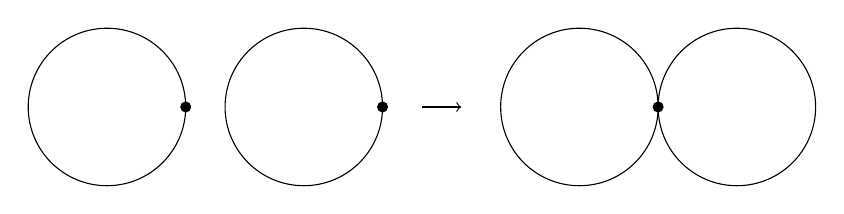
\begin{tikzpicture}
        \draw (-7,0) circle (1);
        \fill (-6,0) circle (2pt);
        \draw (-4.5,0) circle (1);
        \fill (-3.5,0) circle (2pt);
        \draw[->] (-3,0) -- (-2.5,0);
        \draw (-1,0) circle (1);
        \draw (1,0) circle (1);
        \fill (0,0)  circle (2pt);
    \end{tikzpicture}
.\] 
\end{example}

\begin{example}
    Es ist $[0,\frac{1}{2}] \twedge_{\frac{1}{2}} [\frac{1}{2},1] \cong [0,1]$. Verkleben wir allerdings die Punkte $\frac{1}{4}$ und $\frac{3}{4}$, so erhalten wir nicht das Einheitsintervall, sondern ein Plus-Zeichen.
\end{example}

\begin{remark*}
    Aus anderen mathematischen Richtungen kennt man das Wort 'Wedge' eigentlich als Symbol $\wedge$. In der Topologie ist dies jedoch anders. Das Symbol $\tsmash$ heißt 'Smash' und definiert das Smash-Produkt zweier Räume:
     \[
    X \land Y := X \times  Y / X \twedge Y
    .\]  
Es ist z.B. $S^1\tsmash S^1 \cong S^2$ und sogar allgemein $S^n \tsmash S^n \cong S^{2n}$.
\end{remark*}

\begin{gag}
\begin{definition}[Smash-Produkt]\label{def:smash-produkt}
    Seien $X,Y$ topologische Räume und  $x\in X, y\in Y$ Punkte. Dann ist das \vocab{Smash-Produkt} definiert als
    \[
        (X,x) \tsmash (Y,y) = X\times Y / (X\times \left \{y\right\} \cup \left \{x\right\} \times Y)
    .\] 
\end{definition}
\end{gag}


\missingfigure{Torus als Smash-Produkt $S^1 \tsmash S^1$}
\todo{Bruch-nummer hinzufügen}
%%%%%Für die Latex-Nutzer: Ich verwende die Befehle \twedge und \tsmash, um die topologischen wedge und smash- symbole zu erzeugen. Ich bin ein Fan von semantischen Commands, das ermöglich a) sich nicht verwirren zu lassen, wenn man TeXt, wenn man den Code wieder liest etc und vermeidet Konflikte mit anderen Definitionen bzw. Dateien (und verwirrt mich weniger). Außerdem hat es den Vorteil, dass ich jederzeit \twedge und \tsmash neu definieren kann, sollte es nötig sein. Die No tation ist etwas analog zu \land und \lor für 'logic and" und 'logic ar' etc.
\begin{remark*}
    In der Pause stellte sich die Frage, ob es ein Beispiel für einen nicht-normalen Hausdorff-Raum gibt. Siehe hierzu \cite[][Gegenbeispiel 86]{counterexamples}.
\end{remark*}

\begin{example*}[Punktierte Tychonoff-Planke]

    Wir geben (nach einem Kommentar von {\sc Melvin Weiß}) ein Beispiel für einen Hausdorff-Raum, der nicht normal ist, die sogenannte \vocab{gelöschte Tychonoff-Planke} (eng: 'deleted Tychonoff plank'). Sei hierzu $\aleph_0$ die erste unendliche Kardinalzahl und $\aleph_1$ die erste überabzählbare Kardinalzahl. Auf den Räumen $[0,\aleph_0]$ und  $[0,\aleph_1]$ können wir in natürlicher Weise eine Topologie definieren, indem wir die Anfangs- und Endstücke des Intervalls als Subbasis wählen. Der Raum
    \[
        T := [0,\aleph_0] \times [0,\aleph_1]
    .\] 
    heißt Tychonoff-Planke und ist ein kompakter Hausdorff-Raum, also insbesondere normal. Der Teilraum
    \[
        T_{\text{deleted}} := T \setminus \left \{\infty\right\}  := T \setminus \left \{(\aleph_0, \aleph_1)\right\} 
    .\] 
    heißt punktierte Tychonoff-Planke und ist ein lokal kompakter Hausdorffraum, allerdings nicht normal.
    \begin{proof}[Beweisskizze]
        Wir verweisen an dieser Stelle darauf, dass $[0,α]$ für jede Ordinalzahl  $α$ ein kompakter Hausdorffraum ist, das ganze beruht im Wesentlichen darauf, dass die Ordinalzahlen eine Wohlordnung bilden. Also ist  $T$ als produkt von kompakten Hausdorffräumen ebenfalls kompakter Hausdorffraum (\autoref{thm:produkte-von-Hausdorff-Räumen-sind-Hausdorff}, \autoref{thm:tychonoff}), also normal (\autoref{thm:kompakter-hausdorff-raum-ist-normal}. \\
        Der Teilraum $T_{\text{deleted}}$ ist also als Teilraum eines Hausdorff-Raumes ebenfalls Hausdorff. Allerdings lassen sich die beiden abgeschlossenen Mengen
        \[
            A:= [0,\aleph_0) \times \left \{\aleph_1\right\}, \qquad B := \left \{\aleph_0\right\} \times [0,\aleph_1)
        .\] 
        nicht durch offene Mengen trennen: \\
        Angenommen, wir finden $A\subset U$ und $B\subset V$ mit $U,V$ offen. Sei  $n\in \N = \aleph_0$ beliebig, dann ist $(n,\aleph_1)\in A\subset U$. Da $U$ offen, finden wir ein Basiselement der Produkttopologie, das  $(n,\aleph_1)$ enthält, also gibt es  $α_n<\aleph_1$, sodass bereits das Intervall  $\left \{n\right\} \times [α_n, \aleph_1] \subset U$ ist (an dieser Stelle sollte man sich eigentlich genauer Fragen, wie die Topologie auf einer Ordinalzahl definiert ist, die Details, und warum die behauptete Aussage folgt, sind aber leicht zu überlegen). Jetzt kommt der Trick: Wir betrachten
        \[
        β := \sup_{n\in \N} α_n
        .\] 
        \begin{claim}
            $β<\aleph_1$
        \end{claim}
        \begin{subproof}
            Es ist $β = \bigcup_{n\in \N} α_n$ (nach Konstruktion der Ordinalzahlen) wieder eine Ordinalzahl. Da $α_n < \aleph_1$ ist  $α_n$ (als Menge) abzählbar, und somit auch  $β$ als abzählbare Vereinigung abzählbarer Mengen, also ist auch  $β<\aleph_1$, weil  $\aleph_1$ überabzählbar ist.    
        \end{subproof}
        Jetzt wissen wir also, dass sogar der Streifen $[0,\aleph_0) \times [β,\aleph_1]\subset U$ ist (nach Wahl der $α_n$), d.h. die Menge  $U$ enthält sogar ein 'Rechteck positiver Höhe', was absurd ist. Formal können wir argumentieren, indem wir jetzt für den Punkt $(\aleph_0, β)\in B$ eine offene Umgebung wählen und somit ein Intervall $[\gamma, \aleph_0) \times \left \{β\right\} \subset V$ mit $\gamma <\aleph_0$ finden. Dann ist jedoch $(\gamma, \beta)\in U\cap V$, \contra.
    \end{proof}
        Das absurde an dem Beispiel ist, dass wir das Supremum der $α_n$ nehmen, die zwar alle  $<\aleph_1$ sind, aber dennoch  $β \neq \aleph_1$ folgt. Von den reellen Zahlen sind wir gewohnt, dass hier Gleichheit eintreten kann. Wir haben also sogar gezeigt, dass
        \begin{claim}
            Im Raum $[0,\aleph_1)$ konvergiert jede monoton steigende Folge.
        \end{claim}
        \noindent\textbf{obwohl} der Raum nach oben keine Schranke besitzt. Die Moral daran ist ungefähr '$\aleph_1$ ist zu groß, um von Folgen erreicht zu werden'. Das motiviert auch die Einführung von Netzen für größere topologische Räume, die wir hier aber nicht behandeln.
\end{example*}


Wir haben nun Abbildungen $j_i \colon X_i \to  X_1 \bigcup_{X_0} X_2 $:
\[
\begin{tikzcd}
    X_1 \ar[swap]{dr}{j_1} \ar{r}{ι_1}& X_1 \coprod X_2 \ar{d}{q} \\
        & X_1 \bigcup\limits_{X_0} X_2 
\end{tikzcd}
\qquad
\begin{tikzcd}
    X_2 \ar[swap]{dr}{j_2} \ar{r}{ι_2}& X_1 \coprod X_2 \ar{d}{q} \\
        & X_2 \bigcup\limits_{X_0} X_1 
\end{tikzcd}
.\] 
\begin{lemma}\label{lm:injektive-einbettung-ergibt-injetive-projektion-auf-koprodukt-über-basis}
Seien $X_0,X_1,X_2$ topologische Räume, $f_1 \colon X_0 \to  X_1$, $f_2 \colon X_0 \to  X_2$ stetig und betrachte die kanonischen Abbildungen $ι_i\colon X_i \to  X_1 \coprod X_2$ sowie $q : X_1 \coprod X_2 \to  X_1 \bigcup\limits_{X_0} X_2$. \\
Ist $f_1$ injektiv so ist $j_2$ injektiv. Ist  $f_2$ injektiv, so ist $j_1$ injektiv.
\end{lemma}
\begin{proof}
    Wir zeigen nur die erste Aussage, die zweite folgt aus Symmetriegründen. Seien $x,y \in X_2$ mit $j_2(x) = j_2(y)$, nach Konstruktion ist also $x \sim y$. Da die Äquivalenzrelation erzeugt ist von $f_1(x) \sim f_2(x)$, gibt es nun eine Folge von Punkten $x := p_1 \sim  p_2 \sim  \ldots \sim  p_n =: y$, die jeweils von der Form $f_1(x) \sim  f_2(x)$ sind.
    \begin{recap}
        Erzeugen wir eine Äquivalenzrelation durch $x_i \sim  y_i$ für $i\in I$, so sind zwei Element $x,y$ genau dann äquivalent, wenn es eine endliche Folge  $x = a_0 \sim  a_1 \sim  \ldots \sim a_n = y$ gibt, wobei $\left \{a_i, a_{i+1}\right\}  = \left \{(x_i, y_i\right\} $   für ein $i\in I$. 
    \end{recap}
    Genauer gibt es also $x_1\in X_0$ mit $f_2(x_1 ) = p_1 = x$ und $f_1(x_1) = p_2$, und $\exists x_2\in X_0$ mit $f_2(x_2) = p_3$ sowie $f_1(x_2) = p_2$ (auf welcher Seite $f_1$ bzw. $f_2$ steht, ergibt sich daraus, dass die Punkte $p_i$ alternierend aus  $X_1$,$X_2$ kommen müssen). Allgemein gibt es also $x_i \in X_0$ mit 
    \[
        f_2(x_{2i-1}) = p_{2i-1},\quad f_1(x_{2i-1} = p_{2i}),\quad  f_2(x_{2i} = p_{2i+1}),\quad f_1(x_{2i}) = p_{2i} 
    \]
    Nun wissen wir aber, dass $f_1$ injektiv ist, also ergibt sich $x_{2i-1} = x_{2i}$. Dann ist bereits:
    \[
        x = f_2(x_1) = f_2(x_2) = p_3 = = f_2(x_3) = f_2(x_4) = p_5 = \ldots = y
    .\] 
    und damit haben wir $x=y$ gezeigt und  $j_2$ ist wie gewünscht injektiv.
    \missingfigure{Beweisskizze}
\end{proof}

Wir kehren nun zu unserer Ausgangssituation bzw. Ausgangsfrage zurück: \\
Sei $X$ ein topologischer Raum und seien  $X_1,X_2\subset X$ Unterräume, sodass $X_1 \cup X_2 = X$. Setze $X_0 := X_1 \cap  X_2$. \\
Betrachte
    \begin{equation*}
    f': \left| \begin{array}{c c l} 
    X_1\coprod X_2 & \longrightarrow & X \\
    (1,x) & \longmapsto &  x \\
    (2,x) & \longmapsto & x
    \end{array} \right.
\end{equation*}
(im Wesentlichen ist das die Projektion, sodass wir das 'disjunkt' aus der Vereinigung wieder loswerden). Dann faktorisiert $f'$ nach der Universellen Eigenschaft der Quotiententopologie über $f: X_1 \bigcup_{X_0} X_2 \to  X$, dh wir erhalten:
\[
\begin{tikzcd}
    X_1 \coprod X_2 \ar{r}{f'} \ar[swap]{d}{q} & X \\
    X_1 \bigcup_{X_0} X_2 \ar[swap]{ur}{f} 
\end{tikzcd}
\]
Es ist $f'$ surjektiv wegen  $X_1 \cup X_2 = X$, also auch $f'$, und wir prüfen auch leicht die Injektivität von  $f$. Nun ist:

\begin{theorem}\label{thm:raum-ist-koprodukt-über-schnitt-zweier-teilmengen-wenn-diese-offen-oder-abgeschlossen-sind}
    Betrachte die Konstruktion von eben. Nimm an, dass zusätzlich eine der Bedingungen
     \begin{enumerate}[1.]
        \item $X_1,X_2$ sind offen.
        \item $X_1,X_2$ sind abgeschlossen.
    \end{enumerate}
    gilt. Dann ist $f$ ein Homöomorphismus.
\end{theorem}

\begin{proof}
Wir zeigen die Aussage nur unter Verwendung von 2., der Fall 1. geht analog. Es genügt zu zeigen, dass $f$ abgeschlossen ist (weil wir schon wissen, dass  $f$ eine stetige Bijektion ist). Sei  $A\subset X_1\bigcup\limits_{X_0} X_2$ abgeschlossen. Dann sind $j^{-1}_1(A)\subset X_1$ und $j^{-1}_2(A)\subset X_2$ abgeschlossen, da $j_1,j_2$ stetig. Wegen
    \[
        f(A) = j^{-1}_1(A) \cup j^{-1}_2(A)
    .\] 
    sind wir fertig, indem wir ($j^{-1}_1(A)\subset X_1$ abgeschlossen und $X_1\subset X$ abgeschlossen) $\implies j^{-1}_1(A) \subset X$ abgeschlossen bemerken. 
\end{proof}

\begin{remark*}
    Die Stetigkeit von $f^{-1}$ kann man auch mit \autoref{aufgabe-2.2} einsehen, weil $X = X_1 \cup X_2$ mit $X_1,X_2$ abgeschlossen ist, und die entsprechenden Teilabbildungen $X_1 \to X_1 \bigcup_{X_0} X_2$ Einbettungen sind. Im Wesentlichen wiederholen wir hier einfach nur die Aussage des Übungsblattes.
\end{remark*}

\begin{example}
    Sei $X = S^n$ und betrachte die Teilräume  \[
        X_1 = \left \{x\in S^n \mid  x_{n+1}\geq 0\right\} \qquad X_2 = \left \{x\in S^n \mid  x_{n+1} \leq 0\right\} 
    \]
    , also die obere und untere Halbkugel. Der Schnitt
    \[
    X_0 := X_1 \cap  X_2 = \left \{x\in S^n \mid  x_{n+1} = 0\right\} 
    .\] 
    ist dann genau der Äquator der Kugel, also lernen wir aus \autoref{thm:raum-ist-koprodukt-über-schnitt-zweier-teilmengen-wenn-diese-offen-oder-abgeschlossen-sind}, dass
     \[
    S^n \cong X_1 \bigcup_{X_0} X_2 
    .\] 
    Mit der Abbildung
        \begin{equation*}
        \begin{array}{c c l} 
        X_1 & \longrightarrow & D^n \\
        (x_1,\ldots,x_{n+1}) & \longmapsto &  (x_1,\ldots,x_n)
        \end{array}
    \end{equation*}
    (die Projektion auf die $n$-Dimensionale Scheibe) erhalten wir einen Homöomorphismus  $D^n \cong X_1, X_2$, also haben wir eigentlich sogar
    \[
    S^n \cong D^n \bigcup_{S^{n-1}} D^n
    .\] 
    gezeigt.
    \missingfigure{Kugel skizzieren}
    \begin{warning}
        Auch hier ist wieder wichtig, dass wir $S^{n-1}\hookrightarrow D^n$ jeweils kanonisch einbetten, für andere Abbildungen haben wir bereits gesehen, dass wir andere Räume erhalten können.
    \end{warning}
\end{example}




